	The interface for designing questionnaires provides high-level visual tools to facilitate the creation of survey features without needing to write any \gls{xml} code. This permits designers, that usually do not have programming skills, to create simple to complex questionnaire specifications. The interface has two modes: one for describing the content and personalisation features; and the other for specifying the questionnaire's routing.

	Figure \ref{fig:impl:designInterface1} represents the look and feel of the authoring tool for questionnaire specifications. Specifically, this screen shot depicts questions INF1, Q1, Q2, Q3 and Q4 from Figure \ref{fig:background:survey} with a top bottom sequence order. At the top, there are two functionalities that are only applicable for a section. These are, \emph{filter} that permits describing a logical expression and \emph{loop} that allows specifying any of the three iteration modes (e.g. range, list and expr\_list explained in the Section \ref{sec:impl:for}). The right side has a toolbox to access to the global variables (e.g. Variable button) as well as to switch to the content screen (e.g. content button). Next to each question there is a button (e.g. wheel) that allows selecting any routing feature. For instance, the example provided describes three skip constructs (e.g. under Q1, Q2 and Q3) where three combo boxes must be specified: the first combo, it is used to select a response from a question given (e.g. response never from Q1); the second requires to choose a binary operator (e.g. IS\_SEL); and the third expects a destination question (e.g. END). In order to avoid circular dependencies, this interface provides mechanisms that prevents questionnaire designers to define skips to questions defined above this construct on the screen.

	\begin{figure}[h]
	\centering
	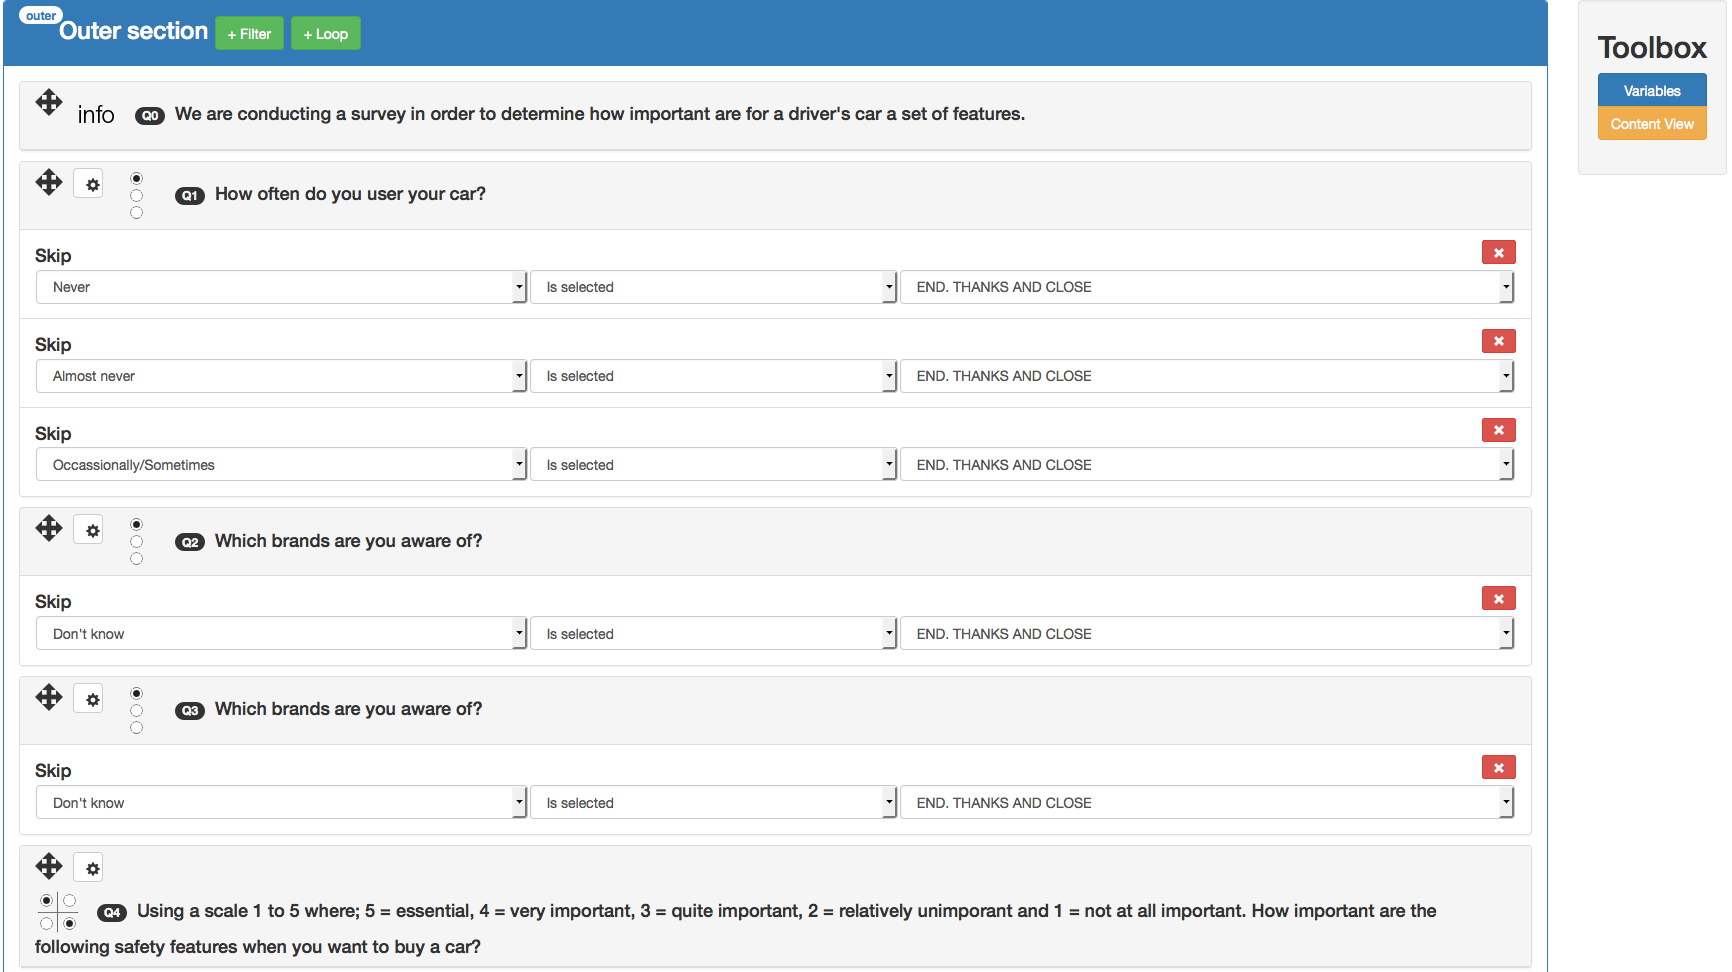
\includegraphics[width=0.90\textwidth]{implementation/img/design_1}
	\caption{Routing design interface}
	\label{fig:impl:designInterface1}
	\end{figure}

	Figure \ref{fig:impl:designInterface2} represents the routing from Q4 till END for the questionnaire Figure \ref{fig:background:survey}. Two constructs are defined; a filter (e.g. over Q5) and an expr\_list loop (e.g. above Q6a). The routing constructs, although are presented in the interface through infix notation mode, are automatically translated to postfix by using the Shunting-yard algorithm \footnote{\url{http://rosettacode.org/wiki/Parsing/Shunting-yard_algorithm\#JavaScript}}. This is mainly due to the fact that \gls{cawiml} only accepts \gls{rpn} expressions for logical and arithmetical operations.

	\begin{figure}[h]
	\centering
	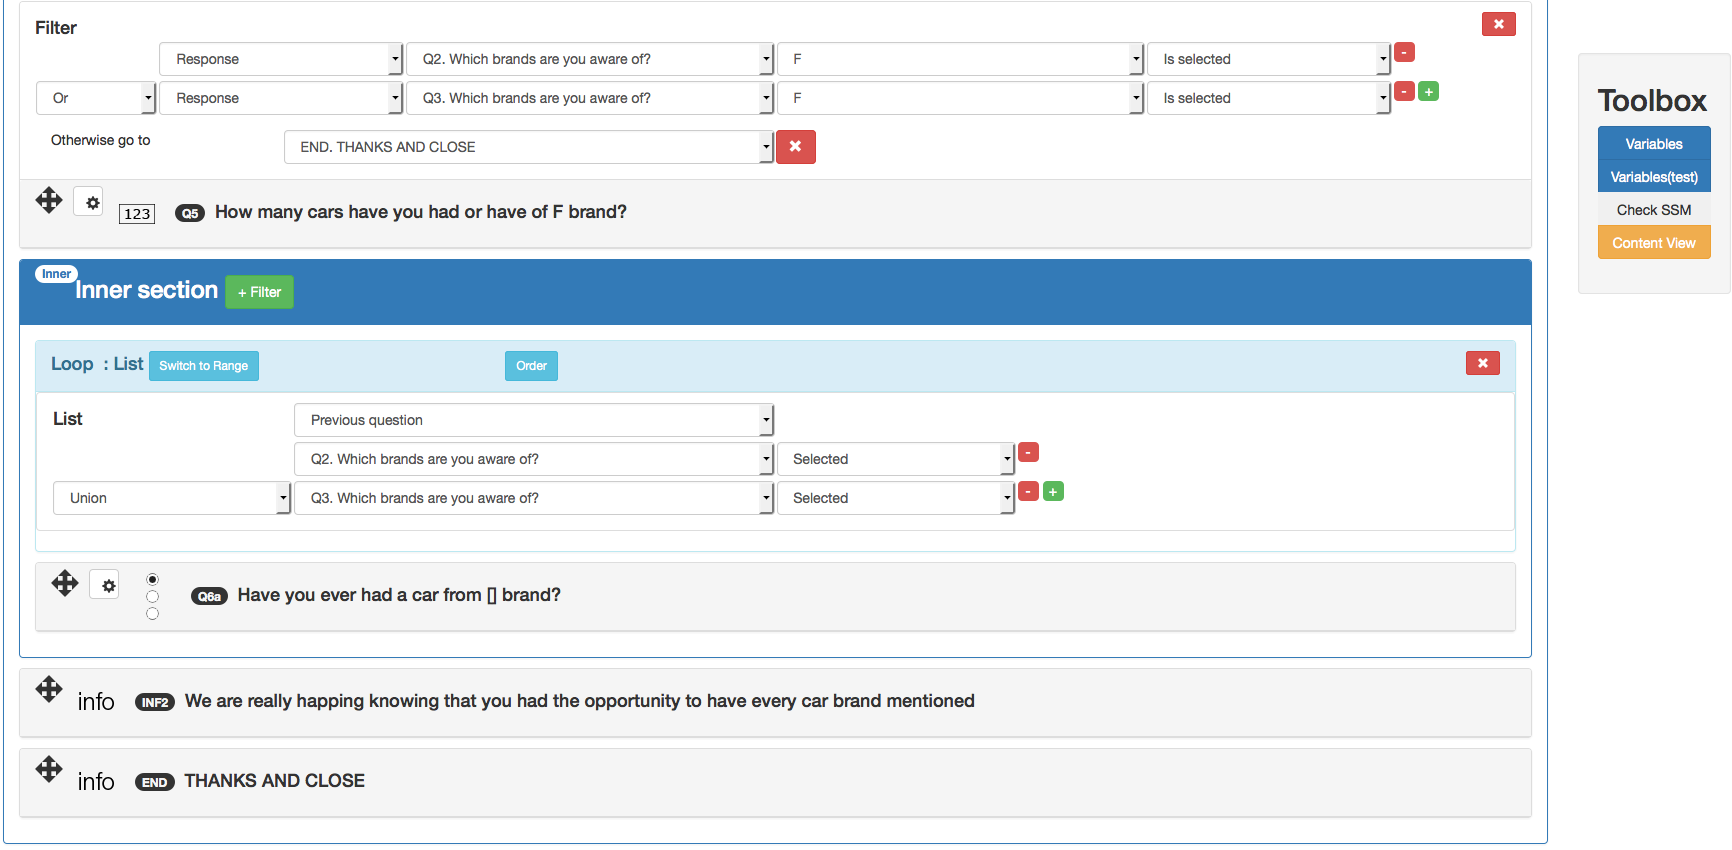
\includegraphics[width=0.90\textwidth]{implementation/img/design_2}
	\caption{Content/Personalisation design interface}
	\label{fig:impl:designInterface2}
	\end{figure}
